\documentclass[11pt,parskip,abstracton,notitlepage, dvipsnames]{scrartcl}

\usepackage{amssymb, amsmath, amsthm, graphics, graphicx, longtable, setspace, makeidx, marvosym, microtype, booktabs, tabularx,authblk, lipsum, siunitx, lmodern, makecell, rotating, pdflscape,fullpage, caption, subcaption, caption, gensymb, multirow, gensymb
}
\usepackage{tikz}
\usetikzlibrary{positioning,chains}
\usepackage[titletoc]{appendix}
\usepackage[hang,flushmargin]{footmisc}
\usepackage[font=footnotesize,labelfont=bf]{caption}
\usepackage[a4paper]{geometry}
\usepackage[T1]{fontenc}
\usepackage{charter}
\usepackage[style=british]{csquotes}
\usepackage{float}
\usepackage[dutch,british]{babel}
\usepackage{dcolumn}
\usepackage{arydshln}
\newcolumntype{d}[1]{D{.}{.}{#1}} 
\newcommand\numberthis{\addtocounter{equation}{1}\tag{\theequation}}

\usepackage[style= authoryear, backend=biber, natbib=true, giveninits=true, uniquename=init,doi=false,isbn=false,url=false, maxnames=2, maxcitenames=2, maxbibnames=10, dashed =true, useprefix=true]{biblatex}
%\DeclareSortingNamekeyTemplate{
%	\keypart{
%		\namepart{family}
%	}
%	\keypart{
%		\namepart{prefix}
%	}
%	\keypart{
%		\namepart{given}
%	}
%	\keypart{
%		\namepart{suffix}
%	}
%}
\AtEveryBibitem{%
	\clearfield{note}%
}
\renewbibmacro{begentry}{\midsentence}
\usepackage{dcolumn}
\renewcommand*{\compcitedelim}{\addsemicolon\space}
\renewbibmacro{in:}{}
\setlength\bibhang{20pt}
\setlength{\footnotemargin}{0.8em}
\bibliography{references}
\AtEveryBibitem{%
	\clearfield{day}%
	\clearfield{month}%
	\clearfield{endday}%
	\clearfield{endmonth}%
}
\onehalfspacing
%\onehalfspacing
\KOMAoptions{DIV=last}
\usepackage[pdftex,colorlinks=true,linkcolor=BlueViolet, citecolor=BlueViolet,urlcolor=BlueViolet,pdfstartview=FitH]{hyperref}
\pdfcompresslevel=9
\hypersetup{pdftitle=Urban exodus or rural shrinkage? Regional migration and attractiveness in a tight Dutch housing market,
	pdfauthor={}}

\begin{document}
	\title{Urban exodus or rural shrinkage? Regional migration and attractiveness in a tight Dutch housing market\thanks{I would like to thank Wim Bernasco, Thor Husby, 		Viktor Venhorst, Maureen Lankhuizen, participants at the 15$^{\text{th}}$ biennial NECTAR conference in
	Helsinki, participants at the 59$^{\text{th}}$ and 60$^{\text{th}}$ ERSA conferences in Lyon and Bolzano (online), 
	seminar participants at the VU University Amsterdam and Wageningen University \& Research for valuable comments on a
	first draft of this paper. Latest versions from paper, data and code can be retrieved from the
	following project's GitHub page: \href{https://github.com/Thdegraaff/migration_gravity}{https://github.com/Thdegraaff/migration\_gravity}. Corresponding author: \url{t.de.graaff@vu.nl.}} }

	\author[1,2]{\small Thomas de Graaff}
	\affil[1]{\small Department of Spatial Economics, Vrije Universiteit Amsterdam, The Netherlands}
	\affil[2]{\small Tinbergen Institute, Amsterdam, The Netherlands}
	
	
	\date{\normalsize \today}
	\maketitle
	
	\begin{abstract}
		\noindent I address the impact of home-ownership and social
		renting rates on regional domestic migration in the Netherlands. I focus
		especially on their relation with natives' migration out of the larger and
		more popular Dutch urban regions. By applying a social relations model I
		am able to control simultanously for (\emph{i}) both region-specific effects
		of origin and destination, (\emph{ii}) dyad (regional pair) specific effects,
		and (\emph{iii}) the impact of the housing market structure in both the region
		of origin and the region of destination. I find positive and high elasticities
		between home-ownership ($1.6$) rates and out-migration and between social renting and in-migration ($0.9$).
		On top of that, I find large positive effects of the largest Dutch urbanised regions on out-migration 
		and I speculate about possible causes. 
		\\
		\\
		{\footnotesize \textbf{Keywords:} housing market, regional domestic migration, social relations model, regional attractiveness
			\newline
			\textbf{JEL-classification:} R23, R31.}
	\end{abstract}
	
	\newpage

\section{Introduction}\label{Introduction}

In the recent decade cities have been proclaimed to be the overall ``winners''
within the regional socio-economic landscape \citep[]{glaeser2012triumph}.
Indeed, there is an abundant empirical literature that finds that especially
large metropolitan areas exhibit---on average---relatively more employment, more
innovation and produce overall more added value \citep[see,
e.g.,][]{balland2020complex}. Most of this success of (large) cities can be
attributed to positive regional and urban agglomeration economies \citep[see for
recent overviews of the size, scope and nature of these urban
economies][]{melo2009meta, duranton2020, rosenthal2020}

Arguably, however, urban benefits do not accrue to everyone equally and recent
empirical research has highlighted the negative sides of the proclaimed urban
success. For example, there is ample empirical evidence of rising levels of
economic segregation witin cities \citep{tammaru2015socio}, of suburbanization
of poverty \citep{hochstenbach2018gentrification}, and crowding out of the
housing market by short-term rentals \citep{koster2018short} and by the
increasing influx of high-skilled migrants to the most popular (inner) cities
\citep{beckers2019residential}.

Indeed, many native residents of large and popular cities are moving out (cite \dots)

Figure \ref{fig:adam_mig} illustrates this by showing out-migration rates of the
urban region of Amsterdam for
various age cohorts in the period 2011--2019. 

\begin{figure}[h!]\centering % Using \begin{figure*} makes the figure take up
  % the entire width of the page
 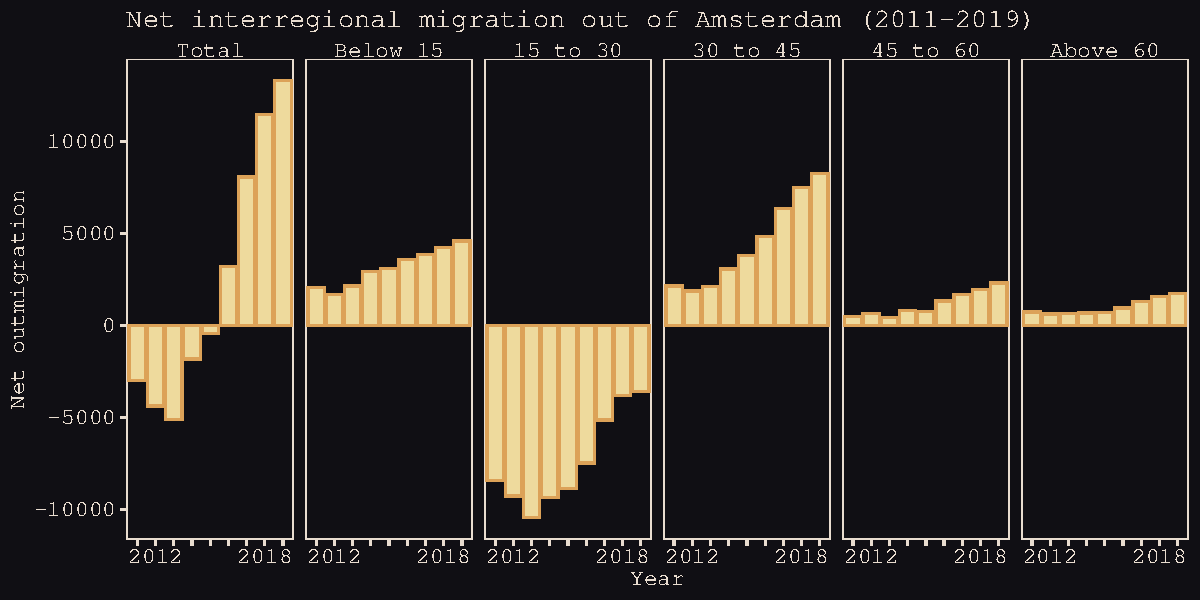
\includegraphics[width=1\linewidth]{../../fig/outmig_amsterdam.pdf}
 \caption{Net domestic regional domestic migration into Amsterdam in the period 2011--2020 for
   various age cohorts (including total population in the most left-panel)}
  \label{fig:adam_mig}
\end{figure}

To anticipate the results of this paper, I find strong negative effects of
home-ownership rates on on both in- and out-migration flows. Further, social
renting rates also affect regional migration flows negatively, but only for
out-migration. So, regions accociated with \ldots

This paper reads as follows. The next section describes the data and focuses
especially on the distribution of regional migration flows and housing market
structure. Section 3 describes the modelling approach, where starting from
traditional gravity model and using the descriptives of the migration flows, a
Bayesian multilevel gravity model is constructed. Section 4 gives both the model
results and interprets them by providing as well predictions within and
out-of-sample. The last section concludes.

\section{Literature}

The current Dutch housing market is characterized by a low housing supply
elasticity, high housing demand, and only a small segment (10\%) that belongs to
the private rental market \citep{michielsen2017}. Because of the resulting large
shortage of housing, many policy recommendations have been proposed, including
plans for 700,000 new houses to be built in the coming decade. Unfortunately,
the construction of a large amount of new dwellings is problematic in the
Netherlands due to large and restrictive spatial constraints
\citep{michielsen2019}. Therefore, policy makers consider as well to change the
housing structure, e.g., by converting rent controlled housing to home-ownership
properties, to tackle at least the high housing prices by enlarging the
home-ownership segment.

There is already a large amount of literature looking into the positive and
negative effects of home-ownership---both from a private and from a social
perspective \citep[see for an overview][]{dietz2003social}. It is argued that
home-ownership leads to, e.g., better maintenance (of the own dwelling and the
neighbourhood), more savings, higher education outcomes, higher individual labor
supply, and even better health. One prominent negative effect of home-ownership
is that it leads to less incentives to move residence because of higher moving
costs vis-\`{a}-vis private renting.

This paper revisits the role of housing market structure as impediment for
inter-municipality migration and specifically focuses on the role of
home-ownership and social renting rates. In addition, it gives a framework to
predict changes in the whole network of migration flows, when housing market
structure change locally. To this end, I adopt a Bayesian multilevel gravity
model which is not frequently encountered in the traditional gravity
literature.\footnote{That is, in the economic literature; a notable exception is
  \citet{ranjan2007bayesian} in the economic trade literature. In the
  geographical literature this approach is more commonly adopted \citep[see
  within a migration context][]{congdon2010random, congdon2012spatial}}
Traditional gravity modelling has the disadvantage that either municipality
fixed effects of origins and destinations can be flows. This paper circumvents
this disadvantage by adopting a multilevel incorporated or the municipalities'
characteristics when not varying over approach with partial
pooling\footnote{There is a whole variety of names for these types of models,
  including hierarchical modeling, varying effects, mixed effects and shrinkage
  models. I use the more generic multilevel description as municipality and
  flows are by definition measured at a different level (scale) \citep[see][for
  an indepth discussion]{gelman2013bayesian}.}, where the latter terms indicates
that I do not impose fixed effects to control for origin and destination
specific effects, but that I ``draw'' them from a distribution, hence the name
partial pooling (where complete pooling states no group effects and no pooling
fixed effects).

This papers adds two main elements to the literature. First, it does not only
consider home-ownership but as well municipal social renting structure, which
can be argued \citep[see, e.g.,][]{hughes1981council,
  boyle1997public,boyle1998migration} to have a large effect on regional
mobility as well as social renting rights are usually only valid locally (within
municipality) and are lost when moving residence between municipalities.

Second, a partial pooling approach has another advantage, namely the municipal
varying effects are completely probabilistic, making it feasible to predict both
within and out-of-sample. In other words, with the results at hand I can predict
migration flows between existing \emph{and} hypothetical cities. The former
might be used for looking at counterfactuals; for example, the changes in
in-migration for all municipalities, when one municipality changes its housing
structure. The latter is useful when one wants to assess new migrations flows
between one or even two new municipalities outside the sample.\footnote{See for
  probabilistic predictions of internation migration \cite{azose2015bayesian}.}

That housing market structure has a sizeable effect on migration decisions is
empirically well-established, especially at the micro-level, where it is widely
accepted that home-ownership has a negative effect on municipal mobility
\citep{dietz2003social, dohmen2005housing}. For example,
\citet{palomares2018understanding} find that home-ownership has a very strong
immobility effect on internal migration in Spain during the period 2001--2011.

In the literature, less attention has been given to inter-city migration on the
aggregate level with respect to the housing market as a specific
barrier.\footnote{See \citet{cushing2004crossing} for a historical overview of
  common themes within migration research.} For the UK,
\citet{congdon2010random} found within a multilevel gravity model that social
rented housing had little effect on the attractivity of a region, although it
had a small positive effect on preventing people from moving residence. For the
Canadian case, \citet{amirault2016drags} looked at the impact of home-ownership
on migration flows within a gravity model using a Poisson pseudo maximum
likelihood estimator and found an elasticity around $-1$.

One of the main reasons to look into housing market structure and migration is
that higher moving costs are detrimental to the aggregate labor market
\citep{oswald1996conjecture, oswald1999housing}. There is a large empirical
literature \citep[see, e.g., ][]{munch2006homeowners, munch2008home,
  de2013european} looking at the impact of individual and aggregate
home-ownership on labour market performance, where seemingly paradoxically at
the aggregate level home-ownership is indeed harmful for labour market behaviour
where at the individual level it is correlated with positive labour market
performance.

This difference between individual and aggregate level is explained by sorting.
Home-owners are indeed less mobile than private renters because of higher fixed
and sunk moving costs which has a negative \emph{aggregate} effect on labour
market performance. However, home-owners are different from renters as they do
\emph{individually} better on the labour market (due to individual unobserved
heterogeneity). So home-owners in countries with high home-ownership rates
perform worse on the labour market vis-\`a-vis home-owners in countries with low
home-ownership rates; but they still perform better than private renters. For
social renters, the effect is different from private renters. On the individual
level they are less mobile than renters at the free market as well, but their
labor market performance is also worse than that of private renters
\citep{hughes1981council, de2009homeownership}.

\section{Modeling framework}

\subsection{The traditional gravity model}

In most disciplines, the workhorse model to study aggregate empirical migration
flows has been the gravity model (see \citet{anderson2011gravity} for a generic
survey of the use of gravity models and \citet{poot2016gravity} for an overview
of migration applications). I therefore start by adopting the basic gravity
model specification pioneered by \citet{tinbergen1962shaping}, so:
\begin{equation}
  \text{migrants}_{ij} = \text{M}_i^{\beta_1}\text{M}_j^{\beta_2}\text{dist}_{ij}^\gamma,
  \label{eq:grav}
\end{equation}
where $\text{migrants}_{ij}$ are the number of migrants moving from $i$ to $j$,
$\text{M}_i$ ($\text{M}_j$) denotes the `mass' of $i$ ($j$), and
$\text{dist}_{ij}$ the distance between $i$ and $j$. Usually, the `mass'
variables are proxied by population, gross domestic product, density, etcetera.
Moreover, the variable $\text{dist}_{ij}$ may represent in general all sorts of
frictions, not only physical distance.

Crucially, \citet{anderson2003gravity} argue that origin and destination
specific variables should be incorporated to take into account multilateral
resistance terms. Most often, this is done by log-linearising model
(\ref{eq:grav} and incorporating fixed effects for origins and destinations, as
follows:
\begin{equation}
  \log(\text{migrants}_{ij}) = o_i + d_j +  \gamma\log(\text{dist}_{ij})
  \label{eq:gravfixed}
\end{equation}
Note that now all origin and destination specific variables are absorbed by the
fixed effects $o_i$ and $d_j$ and that only variables affecting the frictions
$(\text{dist}_{ij})$ can be incorporated, which could be cumbersome if one is
especially interested in those variables.\footnote{If there is another variable
  dimension---say, repeated observations over time---then this problem might be
  circumvented. However, this requires enough variation in the data as
  time-invariant variables can still not be taken into account.}$^{,}$\footnote{An
  often applied strategy to overcome this problem is to use differences between
  origin and destination specific variables. Take for example $\Delta h_{ij}$ as
  the difference in home-ownership rates between $i$ and $j$. A disadvantage of
  this approach is that the difference between 10\% and 20\% home-ownership
  rates and the difference between 80\% and 90\% home-ownership rates would be
  valued as the same.}

\begin{figure}[ht]\centering
  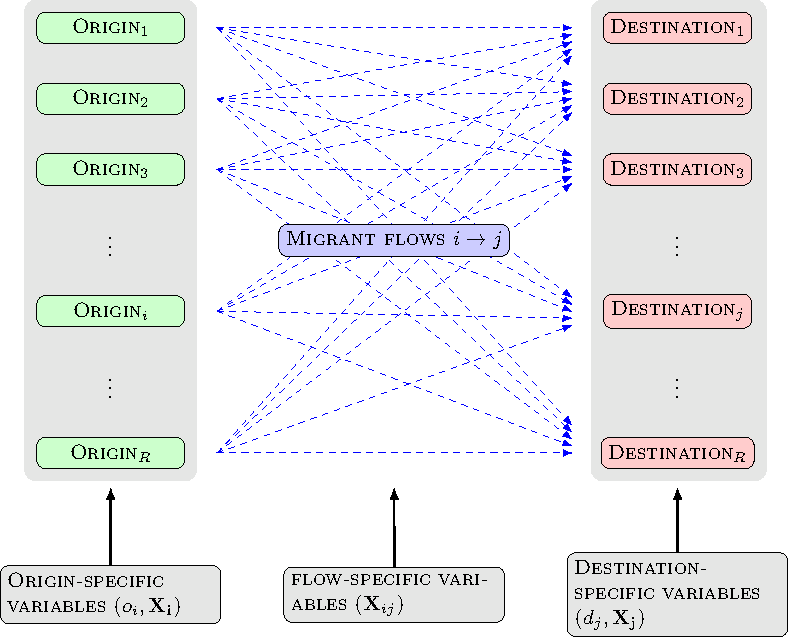
\includegraphics[width=\linewidth]{./../../fig/gravity_network.pdf}
  \caption{Decomposition of variables impacting migration flows from $i$ to $j$
    $\left(\{i,j\} \in \{1,\ldots, R\}\right)$}
  \label{fig:gravity_network}
\end{figure}
Figure \ref{fig:gravity_network} denotes the problem schematically in a generic
dyadic type of network. Typically, one wants to model migration flows between
$i$ and $j$, whilst taken into account both the regional specific effects
($o_i$ and $d_j$) and the regional variables ($\mathbf{X}_i$ and
$\mathbf{X}_j$) one is interested in, such as housing market, population
structure or cultural variables.

Moreover, equation (\ref{eq:gravfixed}) is typically estimated with linear
regression type of models, which is often very cumbersome given the large amount
of zeros migrants flows. `Quick and dirty' remedies as adding a small amount to
the flow variable or removing all zeros have been proven to seriously bias the
results \citep{linders2006estimation, burger2009specification}. An additional problem is that migrant flow data usually suffers from heteroskedasticity---with distributions skewed to the right \citep[][actually states that heteroskedasticity (rather than the presence of too many zeros) is responsible
for the main source of bias within gravity models.]{silva2006log}. For continuous outcome variables a strategy to overcome this is to make use of Pseudo Poisson Maximum Likelihood (PPML) models. If the outcome variable is a count variable one often resorts to negative-binomial models.    

Note that Figure \ref{fig:gravity_network} as well denotes, apart from $\mathbf{X}_{ij}$, country-specific of dyad effects ($\text{dyad}_{ij}$) able to model unobserved region-pair specific effects. Although now frequently used in the trade literature \citep{baier2018heterogeneous, baier2019widely}, incorporating them in a model such as in model (\ref{eq:gravfixed}) requires a large amount of (variation in) panel-data.

To overcome these hurdles, I opt in the next subsection for an alternative strategy which 
can tackle simultaneously issues above: incorporating both city and dyad
varying effects and region and dyad specific variables, controlling for heteroskedasticity and modelling the distribution of migrants flows as they are displayed in Figure \ref{fig:hist_mig_corop}---even when
being zero.

\subsection{A multilevel social relations model for domestic regional migrant flows}

As regional migrant flows are discrete, non-negative and relatively
rare given the size of the population, theoretically the most appropriate way to
go forward is to model migrant flows with a Poisson type of model. To account for the multiplicative nature of the theoretical model as in
(\ref{eq:grav}), I adopt a log link for the expected number of migrants
$\lambda_{ij}$ in the Gamma-Poisson model. Apart from the theoretical model,
note that this log link ensures as well that the expected number of migrants is
always positive. Further, I assume that $\log(\lambda_{ij})$ is a linear
function of the municipal specific variables and the distance between $i$ and
$j$.

To adopt both municipality effects and variables I adopt a multilevel
model with partial pooling. This entails that the regional specific effects
(unlike fixed effects) are now drawn from a, in this case Normal, distribution,
where the parameters of this distribution are estimated as well (in the Bayesian
literature they are known as well as hyper-parameters). Intuitively, this
entails that regions are partially pooled indicating that (statistical)
information between regions is shared. This is an attractive feature, as
fixed effects assume no pooling. In that case, the model only learns from the
information contained in that specific region whereas with partial pooling
it is ensured that outliers (very high or low effects) are effectively
\emph{shrunk} towards the mean. Indeed, this is a further extension of that best
feature of linear regression: regression towards the mean.

Likewise, I adopt a similar strategy for regional pair effects, where I assume
that there is a specific dyad effect for flows from $i$ to $j$ \emph{and} from
flows $j$ to $i$, drawn again from a normal distribution. Together with the
other variables for origins, desinations and flows, the complete model now looks
as follows:
\begin{subequations}
  \begin{align} \text{Migrants}_{ijt} \sim & \text{Poisson}(\lambda_{ijt}), \label{outcome}\\
    \log(\lambda_{ijt}) = & \alpha + o_i + d_j + t_t + \text{dyad}_{ij} + \ln(\mathbf{X}_{it})\beta_1 + \ln(\mathbf{X}_{jt})\beta_2 + \ln(\mathbf{X}_{ijt})\gamma.  \label{model}
  \end{align}
  \label{eq:prefmodel}
\end{subequations}
The first part (\ref{outcome}) models the outcome variable, being the number of
migrants moving from region $i$ to region $j$ in year $t$, using a Poisson distribution
(with parameter $\lambda_{ijt}$). The second part (\ref{model}) states that the
poisson outcome variable is on a log-scale and that the explanatory variables
are on a log-scale as well, allowing for the parameter (vectors) $\beta_1$,
$\beta_2$ and $\gamma$ to be elasticities.
    
As it may well be that, because of unobserved factors, regions are more or less
open for both in- and outmigration, I assume that the regional specific origin,
$o_i$, and destination, $d_j$, variables are correlated as follows:
\begin{equation}
	\begin{pmatrix}o_i\\
		d_j
	\end{pmatrix} \sim \mathcal{N} \left\{\left(\begin{array}{c}
	0\\
	0
       \end{array}\right),
\left(                                        
\begin{array}{cc}
  \sigma^2_i & \rho_{ij} \\
  \rho_{ij} & \sigma^2_{j} 
\end{array}
\right)
\right\}.
\label{eq:randomregion}
\end{equation}
Here, $\sigma_i$ and $\sigma_j$ control the amount of pooling. If they converge
to zero, there is complete pooling and regions of origin and destination come
from the same distribution. If both deviation parameters tend to be very large
(relative to the overall varation in the data), there is no pooling of
regions. Every region of origin and destination is then a separate identity
which should be modeled with the use of fixed effects. When $\sigma_i$ and
$\sigma_j$ are positive and relatively small (again, relative to the overall
variation in the data) there is partial pooling yielding shrinkage: outliers in
the data are effectively shrunk by the model to the overall mean---where the
amount of shrinkage is governed by the size of $\sigma_i$ and $\sigma_j$. The
correlation parameter $\rho_{ij}$ models the correlation between in- and
outflows of regions, as I hypothesize that regions with relatively large amounts
of immigration tend as well to have large amounts of outmigration. Equation (\ref{eq:randomregion}) indicates as well that the region specifi c effects are mean centered around zero, where the final effect can be deduced as deviations around the grand mean $\alpha$.

The dyad specific effects are drawn as well from a multivariate normal distribution as follows: 
 \begin{equation}
	\begin{pmatrix}\text{dyad}_{ij}\\
		\text{dyad}_{ji}
	\end{pmatrix} \sim \mathcal{N} \left\{\left(\begin{array}{c}
	0\\
	0
       \end{array}\right),
\left(                                        
\begin{array}{cc}
  \sigma^2_{\text{dyad}} & \rho \\
  \rho & \sigma^2_{\text{dyad}} 
\end{array}
\right)
\right\},
\end{equation}
where $\sigma^2_{\text{dyad}}$ denotes again the amount of partial pooling at
the dyad level. Note that for dyadic relationship it does not matter whether
flows go from $i$ to $j$ of from $j$ to $i$. Moreover, parameter $\rho$ measures
whether the size of flows from $i$ to $j$ correlates with the size of flows from
$j$ to $i$. Given the tight Dutch housing market in the Netherland, this is more than likely as houses tend not to be vacant very long.

Finally, to control for year specific effects, we include a year varying effect, $t_t$, drawn from a normal distribution as follows: $t_t \sim \mathcal{N}(0, \sigma_t$). 

\section{Data and methods}

\subsection{Data}

I use interregional migration flows measured in individuals migrating between
all of the 40 Dutch COROP regions between 2012 and 2020. I use the period
2012--2019 for estimation and the year 2020 for out-of-sample
forecasting.\footnote{The year 2020 is obviously a strange year containing the
  start of the COVID-19 outbreak in March 2020. I delibarately choose not to
  incorporate this year at it might affect the results, and at the same time
  out-of-sample prediction might contain evidence whether COVID-19 truly changed
  migration patterns.} I use no information on within regional migration. So, I
have 320 time-varying regional characteristics (or doubled when accounting for
both origin and destination municipalities) and 12,480 aggregate migration flows
($8 \times (40 \times 40 - 40)$).

 \begin{figure}[ht]\centering 
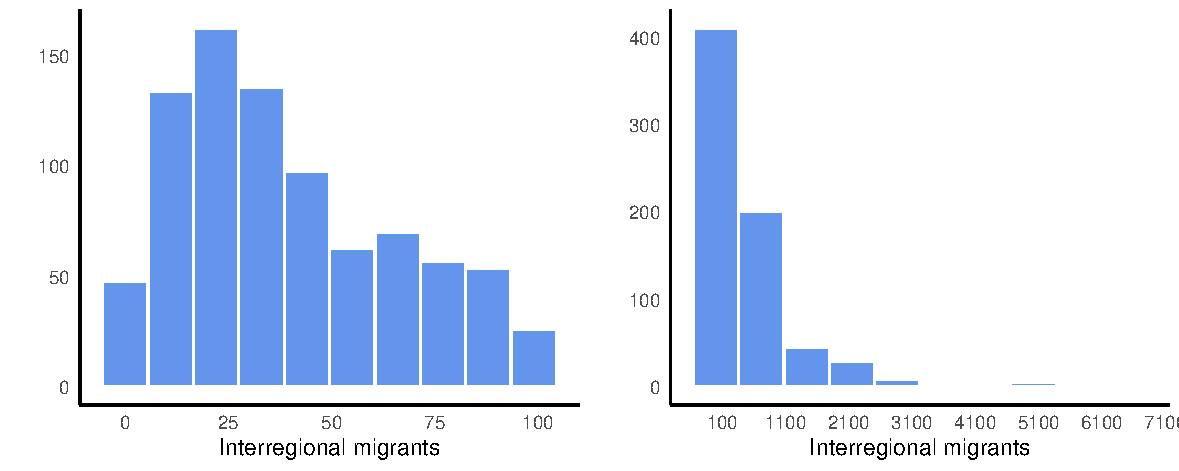
\includegraphics[width=1.0\linewidth]{./../../fig/hist_mig_corop.pdf}
          \caption{Histogram of domestic interregional migrant flows. Left panel
shows the histogram of small migrant flows ($0 \leq N < 100$) and the right
panel shows the histogram of large migrant flows ($N \geq 100$). Note the
different scale of the y-axes.}
\label{fig:hist_mig_corop}
\end{figure}

The histograms in Figure \ref{fig:hist_mig_corop} show the distribution of
migrant flows within the sample. The left panel deals with migrant flows below
100, the right panel with migrant flows of 100 and larger. Two main observations
can be made. First, there is a strong but consistent decay pattern in migration
flow size in both panels, which points to a persistent underlying
pattern. However, the right `tail' in this distribution is rather
thick.\footnote{The largest migration flows are between the urban regions of
  Amsterdam and Utrecht and amount to 7,327 migrants in 2019.} In effect, this entails that there are
still observations quite far right in the distribution. Indeed, the sample mean
is about 273, while the sample variance is around 300,000, leading to a strong
presence of \emph{overdispersion} (unconditional on other explanatory
variables). Second, a small part of the dataset consists of zero
observations. Although they do seem to be genuine observations and not caused by
another process, I check in a robustness analysis whether the occurrence of
zeros does need to be taken specifically into account.

Seven explanatory variables are added to the model. First, to account for
spatial distance decay between origin $i$ and destination $j$, distance between
all regions are calculated as Eucledian distance between regional centroids
($\text{dist}_{ij}$). Secondly, as regional mass we use population size for
both region of origin and region of destination (so $\text{pop}_i$ and
$\text{pop}_j$). Finally, for housing market structure we use variables
indicating percentage of homeownership ($\text{home}_i$ and $\text{home}_j$) and
percentage of social renting ($\text{soc}_i$ and $\text{soc}_j$), again in both
regions of origin and destination. Social renting in the Netherlands includes all
kinds of rent controlled housing but typically involves local housing
corporations offering housing to lower income households, where eligibility is
based on (local---within region) waiting lists.

\begin{figure}[ht]\centering % Using \begin{figure*} makes the figure take up the entire width of the page
  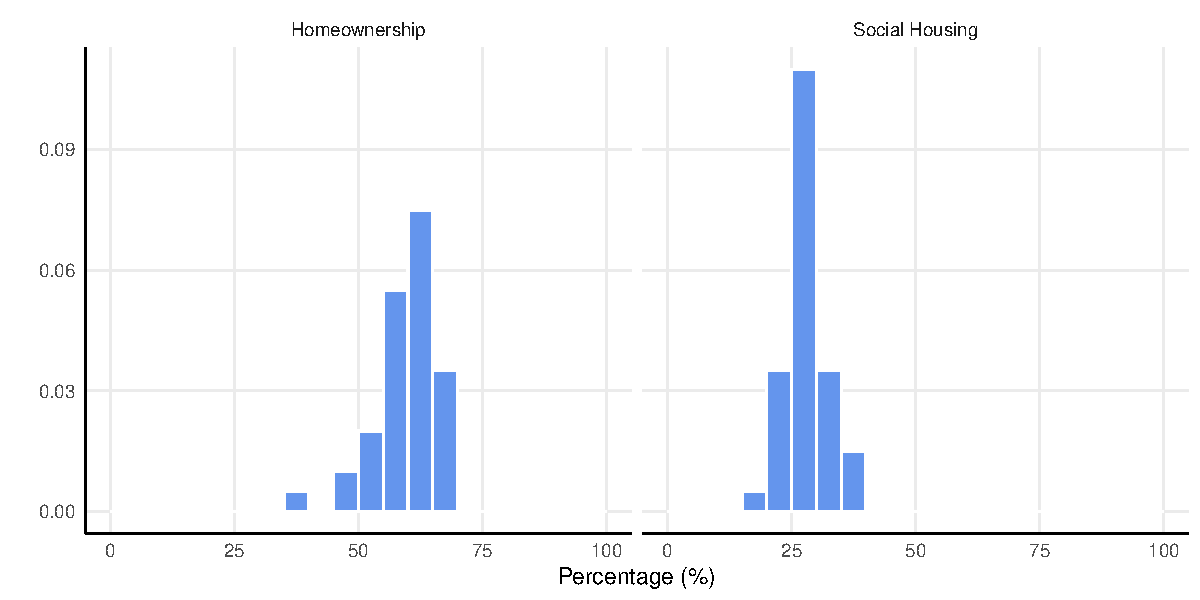
\includegraphics[width=1.0\linewidth]{./../../fig/hist_housing_corop.pdf}
  \caption{Histogram of homeownership (left) and social housing (right)
    percentages in Dutch COROP regions in 2018}
  \label{fig:housing_mig}
\end{figure}

Figure \ref{fig:housing_mig} shows the distribution of social renting and
homeownership across Dutch regions in 2018. Clearly, both homeownership
and social housing are prevalent across Dutch regions, with an average
per region of 25\% of social housing and around 60\% of homeownership. In the last decade, these numbers have been quite robust. Percentage homeownership grew in the period 2012--2020 with only a 0.5 percentage point, while social renting decreased with 1.5 percentage point. Within regions these numbers are less stable. For example, in the region of Amsterdam social renting decreased from 0.39 percent to 0.35 percent of total housing stock.

\begin{figure}[ht]\centering % Using \begin{figure*} makes the figure take up the entire width of the page
  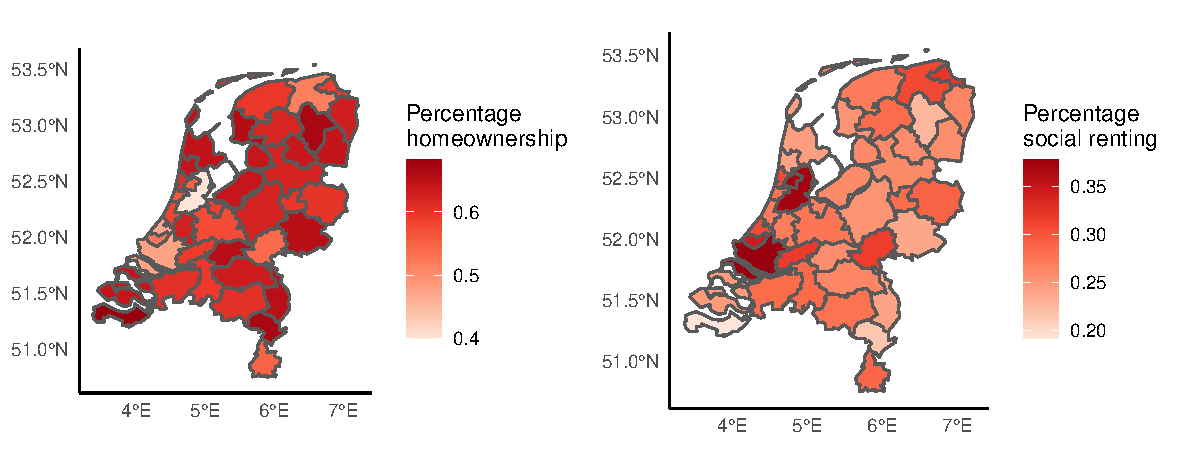
\includegraphics[width=1.0\linewidth]{./../../fig/housing_types.pdf}
  \caption{Maps of homeownership (left) and social housing (right)
    percentages in Dutch COROP regions in 2018 }
  \label{fig:housing_types}
\end{figure}

Figure \ref{fig:housing_types} shows the regional distribution of social renting
and homeownership in 2018. Clearly, social renting is especially prevalent in
the larger urban regions with a correlation of 0.46 between regional size and social
renting (e.g., Amsterdam has about a 37\% social renting rate in 2018). Also,
more rural Dutch regions exhibit much less social renting. Homeownership and
regional size correlate negatively ($-0.63$). Finally, the maps show as well that
there is a large negative correlation between social renting and homeownership
($-0.88$) across regions.

\subsection{Modeling strategy}

For my main estimation, I construct four baseline models, where the first is the most basic gravity model as presented in equation (\ref{eq:grav}) but then with a log-link and using a Poisson distribution on the outcome and the fourth the preferred and most complete specification as presented in equation (\ref{eq:prefmodel}).

So, the first model is specified as:
\begin{align} \text{Migrants}_{ij} \sim & \text{Poisson}(\lambda_{ijt}), \notag \\
  \log(\lambda_{ijt}) = & \alpha +
                          \beta_1 \ln(\text{pop}_{it}) +
                          \beta_2 \ln(\text{pop}_{jt}) +
                          \gamma \ln(\text{dist}_{ijt}),  
\tag{model 1}\label{eq:m1}
\end{align}
where the parameters are still to be interpreted as elasticities.

the second model allows for regional housing market structure:
\begin{align} \text{Migrants}_{ij} \sim & \text{Poisson}(\lambda_{ijt}), \notag \\
  \log(\lambda_{ijt}) = & \alpha + \beta_1 \ln(\text{pop}_{it}) + \beta_2
                          \ln(\text{pop}_{jt}) +
                          \gamma \ln(\text{dist}_{ijt}) + \notag \\
                                        & \beta_3 \ln(\text{home}_{it}) +
                                          \beta_4 \ln(\text{home}_{jt}) +
                                          \beta_5 \ln(\text{soc}_{it}) + \beta_6
                                          \ln(\text{soc}_{jt}). \tag{Model
                                          2} \label{eq:m2}
\end{align}

The third model adds origin and destination regional varying effects to model (\ref{eq:m2}), as well as time-varying effects:
\begin{align} \text{Migrants}_{ij} \sim & \text{Poisson}(\lambda_{ijt}), \notag \\
  \log(\lambda_{ijt}) = & \alpha +  o_i + d_j + t_t + \notag \\
                                        &\beta_1 \ln(\text{pop}_{it}) + \beta_2
                                          \ln(\text{pop}_{jt}) +
                                          \gamma \ln(\text{dist}_{ijt}) + \notag \\
                                        & \beta_3 \ln(\text{home}_{it}) +
                                          \beta_4 \ln(\text{home}_{jt}) +
                                          \beta_5 \ln(\text{soc}_{it}) + \beta_6
                                          \ln(\text{soc}_{jt}).  \tag{Model
                                          3} \label{eq:m3}
\end{align}
Note that the constant, $\alpha$, denotes the grand mean and that regional and time varying effects deviate around that.

Finally, the fourth and preferred model adds dyad specific effects to model (\ref{eq:m3}):                                          
  \begin{align} \text{Migrants}_{ij} \sim & \text{Poisson}(\lambda_{ijt}), \notag \\
    \log(\lambda_{ijt}) = & \alpha +  o_i + d_j + t_t + \text{dyad}_{ij}+ \notag \\
                                          & \beta_1 \ln(\text{pop}_{it}) +
                                            \beta_2 \ln(\text{pop}_{jt}) +
                                            \gamma \ln(\text{dist}_{ijt}) + \notag \\
                                          & \beta_3 \ln(\text{home}_{it}) +
                                            \beta_4 \ln(\text{home}_{jt}) +
                                            \beta_5 \ln(\text{soc}_{it}) +
                                            \beta_6
                                            \ln(\text{soc}_{jt}). \tag{Model
                                            4} \label{eq:m4}
\end{align}

As models (\ref{eq:m1})--(\ref{eq:m4}) are estimated with Bayesian Markov Chain Monte Carlo methods, all parameters can be given priors.\footnote{It is also possible to give parameters flat priors, essentially reducing the models to maximum likelihood models.} Based on previous literature and data descriptives we assume $\alpha$ to be $\mathcal{N}(4,2)$, $\gamma$ to be $\mathcal{N}(-1.5,1)$, $\beta_1$ and $\beta_2$ to be $\mathcal{N}(1, 0.5)$, and $\beta_3$--$\beta_6$ to be $\mathcal{N}(0,1)$ distibuted. All variation parameters ($\sigma_i$, $\sigma^2_{\text{dyad}}$ and $\sigma_t$) are assumed to be exponentially distributed with parameter 1, mainly to ensure a positive standard deviation whilst the tails are still relatively flat. The correlation parameters, $\rho_{ij}$ and $\rho$, are assumed to follow a LKJ(2) distribution which ensures a relatively low probability mass close to the extremes ($-1$ and $1$) \citep{lewandowski2009generating}.\footnote{Although the priors on the standard deviation and correlation parameters are important as they ensure that restrictions on those parameters are satisfied, the priors on the $\alpha$, $\beta$ and $\gamma$ parameters are in this case less essential given the relatively large number of observations.}

To measure model performance I look both at an in-sample and an out-of-sample indicator. For in-sample I simply adopt the R$^2$, measured as the explained sum of squares divided by the total number of squares.\footnote{This R$^{2}$ might deviate a bit from the R$^2$ in standard regression models as the prior distribution adds uncertainty as well, which in the extreme case might yield values higher than one \citep{gelman2019r}. However, given the large number of observations and the relative conservative prior distributions, potential deviations in R$^2$ are minimal.} For out-of-sampling prediction accuracy, we adopt the Leave-One-Out (LOO) cross validation with Pareto Smoothed Importance Sampling (PSIS) presented by \citet{vehtari2017practical}---usually abbreviated to PSIS-LOO---which offers both a robust and efficient (relatively fast) computation. Predictive accuracy improves with lower PSIS-LOOs.

Finally, to assess model performance out-of-sample visually I correlate predictions for regional migration flows in 2020 with actual regional migration flows, which allows me as well to see whether COVID-19 had a large impact on residential migration flows. 

\subsection{Estimation}

I fit models (\ref{eq:m1})--(\ref{eq:m4}) with Markov Chain Monte Carlo sampling provided by the STAN platform for statistical modeling \citep{gelman2015stan}, more notably its implementation in the statistical software package R \citep{r2021, rstan2020}. For data wrangling, coding and visualisation I follow \citet{mcelreath2020statistical} and \citet{kurzStatisticalRethinkingSecondEd2021}. All models are run with 4 chains, each with 4,000 iterations and a warm-up sample of 1,000. Model diagnostics for all models are deemed satisfactorily as each parameter has a large effective sample size (usually more than a 1,000) and has a $\widehat{R}$ at least smaller than $1.05$ (but usually very close to 1) indicating convergence \citep{vehtari2019rank}.

\section{Results}

The results of fitting baseline models (\ref{eq:m1})--(\ref{eq:m4}) are given in Table \ref{table:results}. 

\begin{table}[t!]
\begin{center}
	\begin{footnotesize}
		\begin{longtable}{@{} p{0.20\linewidth} @{\extracolsep{\fill}} D{.}{.}{3.6} D{.}{.}{3.6} D{.}{.}{3.6} D{.}{.}{3.6} }
			\caption{Estimation results---Baseline models (standard errors between parentheses))}
			\label{table:results}\\
			\toprule
			Variable & \multicolumn{1}{c}{\ref{eq:m1} } & \multicolumn{1}{c}{\ref{eq:m2} } & \multicolumn{1}{c}{\ref{eq:m3} } & \multicolumn{1}{c}{\ref{eq:m4} } \\
			\midrule
			\endfirsthead
			\multicolumn{5}{c}%
			{\tablename\ \thetable{} -- continued from previous page} \\
			\toprule 
			Variable & \multicolumn{1}{c}{\ref{eq:m1} } & \multicolumn{1}{c}{\ref{eq:m2} } & \multicolumn{1}{c}{\ref{eq:m3} } & \multicolumn{1}{c}{\ref{eq:m4} } \\
			\midrule
			\endhead
			\midrule 
			\multicolumn{5}{r}{{Continued on next page}} \\ 
			\endfoot
			\midrule
			\endlastfoot
			\bottomrule
			\multicolumn{5}{l}{\scriptsize{$^{***}p<0.01$; $^{**}p<0.05$; $^{*}p<0.1$}}\\
			\endlastfoot
$\alpha$     & 4.793^{***}  & 4.777^{***}   & 4.595^{***}  & 4.490^{***}  \\
			 & (0.001)      & (0.001)       & (0.176)      & (0.164)      \\			
$\ln(\text{dist}_{ijt})$      & -1.345^{***} & -1.385^{***}  & -1.686^{***} & -1.628^{***} \\
             & (0.001)      & (0.001)       & (0.001)      & (0.024)      \\
$\ln(\text{pop}_{it})$     & 0.790^{***}  &  0.770^{***}  & 0.319^{***}  & 0.318^{***}  \\
& (0.001)      &  (0.001)      & (0.033)      & (0.033)      \\             
$\ln(\text{pop}_{jt})$   & 0.827^{***}  &  0.843^{***}  & 0.516^{***}  & 0.549^{***}  \\
             & (0.001)      & (0.001)       & (0.031)      & (0.032)      \\
$\ln(\text{soc}_{it})$        &              & -1.821^{***}  & -0.245^{***} & -0.259^{***} \\
	&              & (0.007)       & (0.055)      & (0.054)     \\
$\ln(\text{home}_{it})$        &              & -1.670^{***}  & 1.575^{***}  & 1.601^{***}  \\
             &              & (0.008)       & (0.088)      & (0.086)     \\
$\ln(\text{soc}_{jt})$         &              & -1.474^{***}  & 0.867^{***}  & 0.867^{***}  \\
             &              & (0.007)       & (0.054)      & (0.054)      \\
$\ln(\text{home}_{jt})$        &              & -1.143^{***}  & 0.169^{**}   & 0.166^{**}   \\
             &              & (0.008)       & (0.086)      & (0.087)      \\
\midrule
hyperparameters:\\
\qquad$\sigma_t$     &              &               & 0.125^{***}  & 0.125^{***} \\
             &              &               & (0.046)      & (0.042)     \\
\qquad$\sigma_i$  &              &               & 0.656^{***}  & 0.673^{***} \\
            &              &               & (0.073)      & (0.082)     \\
\qquad$\sigma_j$  &              &               & 0.466^{***}  & 0.441^{***} \\
             &              &               & (0.053)      & (0.053)     \\
\qquad$\rho_{ij}$     &              &               & 0.803^{***}  & 0.781^{***} \\
             &              &               & (0.060)      & (0.070)     \\
\qquad$\sigma_\text{dyad}$     &              &               &              & 0.385^{***} \\
             &              &               &              & (0.009)     \\
\qquad$\rho$    	 &              &               &              & 0.804^{***} \\
             &              &               &              & (0.014)     \\
\midrule
PSIS-loo    & 849,398   & 793,476   & 384,369   & 123,396   \\
R$^2$           & 0.67        & 0.70        & 0.79        & 0.84        \\
\bottomrule
\end{longtable}
\end{footnotesize}
\end{center}
\end{table}

With two thirds of all variation explained, the first column of Table \ref{table:results} shows that in-sample accuracy of \ref{eq:m1} is already quite high---which again shows the strong explanatory performance of empirical gravity models. The parameters for population of origin and destination and for the distance-decay effect are in the range of what has been found in the previous literature and are very precisely measured with standard errors around $0.001$. Adding housing market structure as in column \ref{eq:m2} both improves in-sample and out-of-sample performance and are parameters remain very precisely measured. Noteworthy is that \ref{eq:m2} shows very negative results for social renting and home-ownership in regions of origin and destination, with elasticities well below $-1$. So, according to \ref{eq:m2} home-ownership and social renting indeed deteriorates  regional Dutch mobility as argued by \citet{oswald1996conjecture, oswald1999housing}. 

However, when allowing for regional varying effects of origin and destination as in column \ref{eq:m3}, the impact of regional housing structure changes drastically. All elasticities decrease in size and three out of four become positive. Most notably, the impact of home-ownership at the origin has a very large and positive elasticity of around $1.6$, followed in size by the percentage social renting in the region of destination which has an elasticity of around $0.9$. The other two elasticities become much smaller than in \ref{eq:m2}. So, when controlling for regional origin and destination varying effect, the negative impact of home-ownership and social renting largely disappears pointing to the existence of unobserved regional factors negative correlated with both home-ownership and social renting. In section \ref{sec:discussion} I speculate on the type and nature of these factors. Note as well that with the inclusion of origin and destination varying effects the other parameters are fitted less precisely, indicating that the model become less certain about the impact of population or housing structure.

Finally, column \ref{eq:m4} yields the results of our preferred model, where most parameters are more or less comparable with the findings of \ref{eq:m3} much in-sample and especially out-of-sample performance is to be preferred over \ref{eq:m3}. Therefore, the remainder of our discussion will use the findings of \ref{eq:m4}. 

To start, Table \ref{table:results} shows that the hyperparameters $\sigma_i$ and $\sigma_j$ are relatively large, indicating a large regional variation in regional specific origin and destination effects. To illustrate this regional variation, the regional varying effects are depicted in Figure \ref{fig:attractivity}. 

\begin{figure}[ht]\centering % Using \begin{figure*} makes the figure take up the entire width of the page
  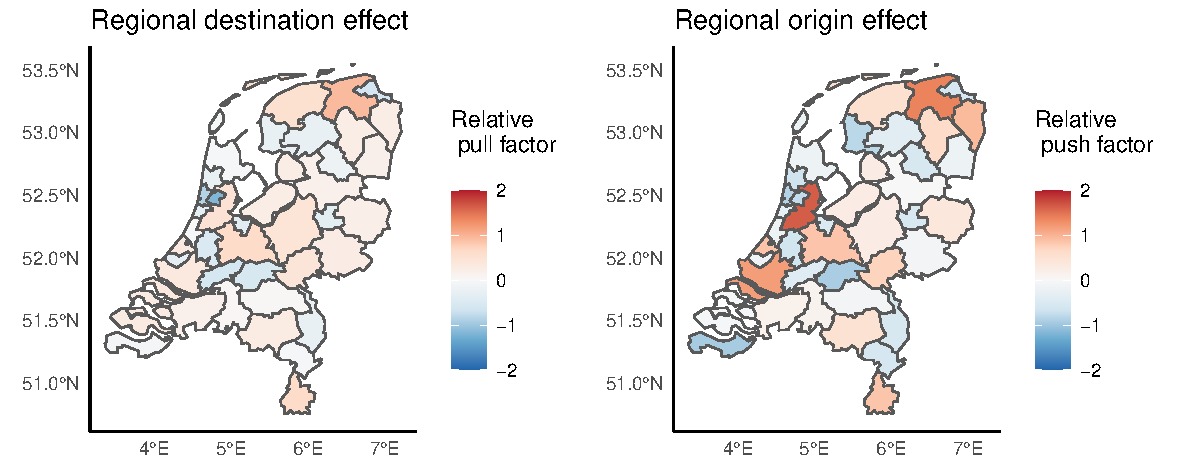
\includegraphics[width=1.0\linewidth]{./../../fig/attractivity_region.pdf}
  \caption{Maps of regional pull/destination (left panel) and push/origin (right panel) factors in Dutch COROP regions in the period 2012--2019.}
  \label{fig:attractivity}
\end{figure}

The left map of \ref{fig:attractivity} shows the relative pull factor across Dutch regions in the period 2012--2019. \citet{congdon2010random} labeled these regional varying effects as measures of attractiveness. However, as especially the region in the north lights up red (which is partly seen as a shrinkage region), attractiveness is a strange concept in a tight housing market. It may as well indicates the availability and affordability of more or less suitable dwellings if one is compelled to move residence. Note as well that the remainder of the country is relatively homegeneous in its pull factors. That is unlike the general push factor in the right panel. Again, the same region in the North lights up red (and even more so than in the left panel)---indicating a relatively large amount of housing dynamics as in the region the housing market is still less tight. However, the largest urban regions in the Netherlands, Amsterdam, Rotterdam, The Hague and Utrecht, light up red as well (especially the urban region of Amsterdam), pointing at the relatively high out-flow of natives. 

\begin{figure}[ht]\centering % Using \begin{figure*} makes the figure take up the entire width of the page
  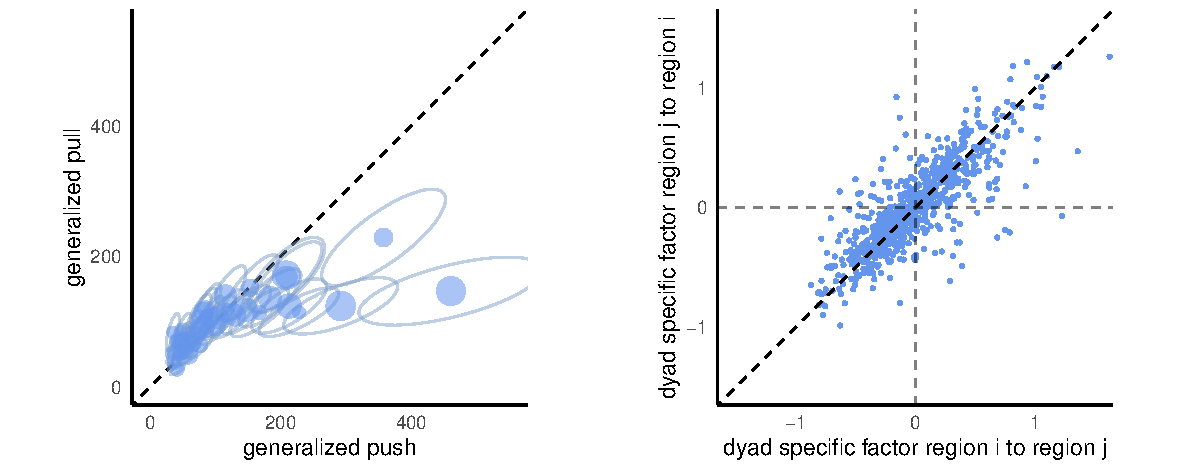
\includegraphics[width=1.0\linewidth]{./../../fig/country_dyad.pdf}
  \caption{Scatterplot between regional generalized push and pull factors, where the size of the circle indicates the population size of the region  (left panel) and scatterplot between dyad specific factors indicating flow from $i$ to $j$ and from $j$ to $i$.}
  \label{fig:correlation}
\end{figure}

The left panel in Figure \ref{fig:correlation} denoting the correlation between generalized pull and pull factors confirms this pattern.\footnote{Generalized push and pull in this case mean that the regional varying effects are combined with the grand mean $\alpha$ and transformed to the outcome scale---being the number of migrants.} Note that the size of the circle is relative to the size of the population. So, where most of the (smaller) regions have more or less similar in- and outflows, it is especially the larger urban areas (together with some peripheral regions), where outflow dominates inflow. Note the high correlation ($\rho_{ij}$) of $0.78$ between the two. Regions that have a high influx of domestic migrants also tend to have a high outflow. Similarly, the right panel shows the high correlation ($\rho = 0.8$) between dyadic pair flows. Thus, if---for whatever reason---the migrant flow from $i$ to $j$ is large, then the reverse migrant flow from $j$ to $i$ is most likely large as well. Interestingly, the inclusion of dyadic correlation does not influence the dyad distance variable as much as the inclusion of region specific varying effects has on the region specific variables as population and housing structure. 

Finally, to assess the extent of predictive accuracy of \ref{eq:m4}, I correlate predicted migrant flows with observed migrant flows in 2020 in Figure \ref{fig:pred}.
\begin{figure}[ht]\centering % Using \begin{figure*} makes the figure take up the entire width of the page
  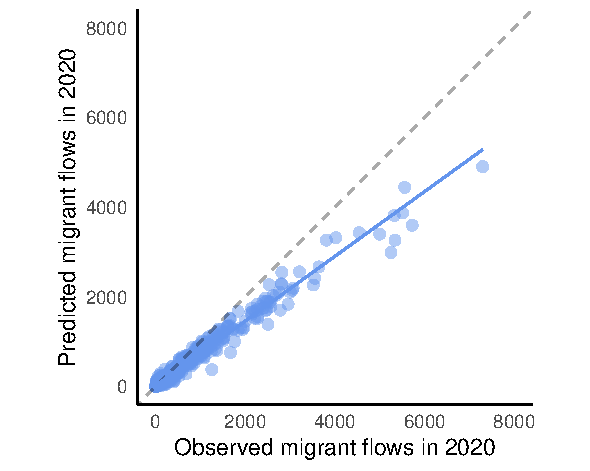
\includegraphics[width=0.5\linewidth]{./../../fig/prediction_2020.pdf}
  \caption{Scatterplot of observed migrant flows versus predicted migrant flows in 2020 flows with associated regression line}
  \label{fig:pred}
\end{figure}
Clearly, predictive accuracy is rather high with the correlation being 0.98 between observed and predicted migrant flows. Interestingly, the regression line lies below the 45\degree line. So, the model is more skeptical about larger values and, indeed, tend to shrink them. Finally, I would like to emphasize that the out-of-sample prediction year is 2020, an exceptional year with the outbreak of COVID-19 in March of that year. But, despite the pandemic with its associated lock-downs, increased working from home rates, diminished trade, and so forth, in terms of (patterns of) Dutch residential migration it turned out not to be exceptional at all. 

To further prove this point, Figure \ref{fig:hist_pred} shows the histograms of observed and prediction migration flows in 2020. Again, the same pattern arises. Apart from the fact that the model is more optimistic about smaller flows and more skeptical about larger flows, the model seems to be able to mimic the whole distribution of residential migration flows to a large extent. 

\begin{figure}[ht]\centering % Using \begin{figure*} makes the figure take up the entire width of the page
  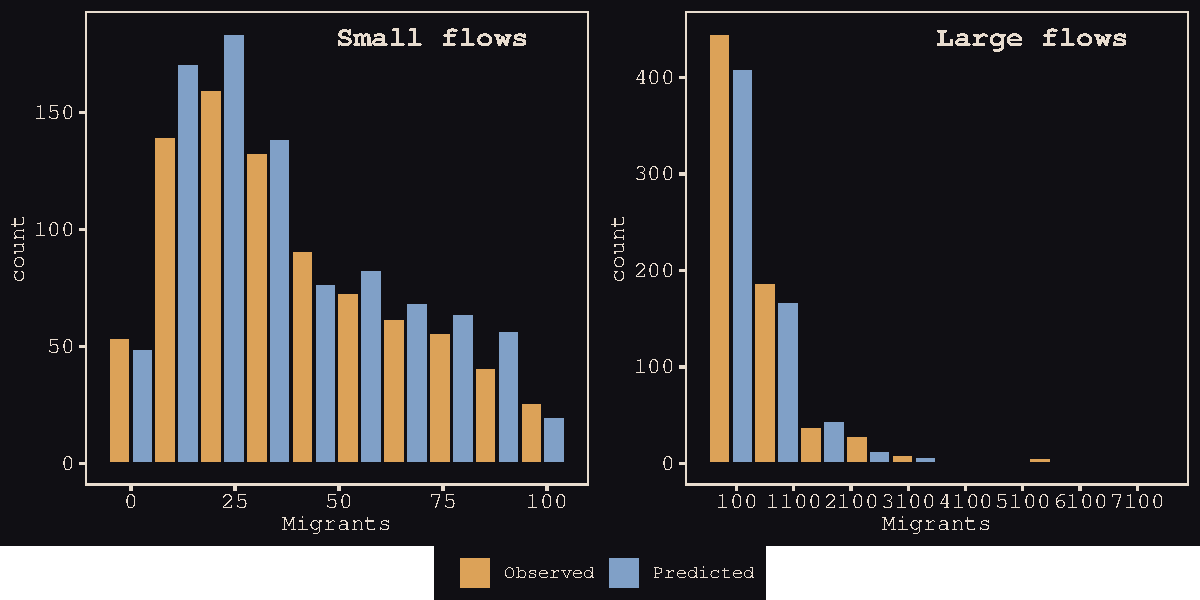
\includegraphics[width=1.0\linewidth]{./../../fig/hist_fit.pdf}
  \caption{Histogram of observed and predicted migration flows in 2020. The left panel shows small flows, the right panel large flows (note the difference in scaling on the axes.)}
  \label{fig:hist_pred}
\end{figure}

\subsection{Spatial correlation\label{subsec:spatial}}

\section{Discussion\label{sec:discussion}}

\begin{figure}[ht]\centering % Using \begin{figure*} makes the figure take up the entire width of the page
	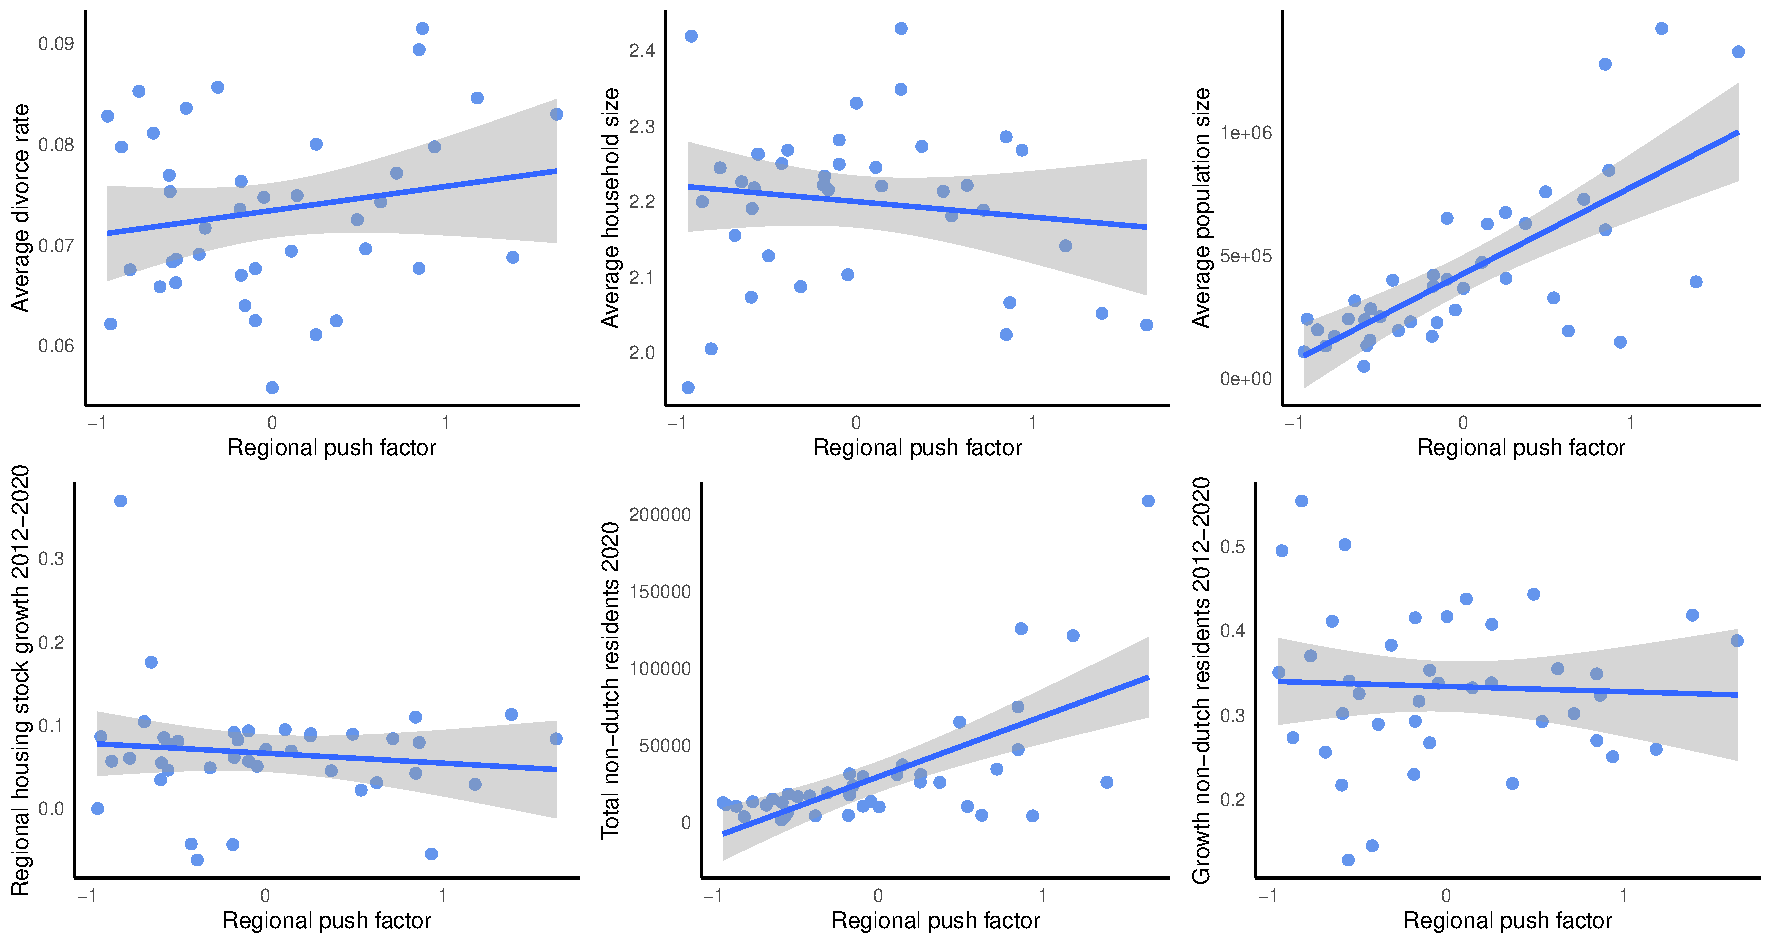
\includegraphics[width=1.0\linewidth]{./../../fig/regional_out_plot.pdf}
	\caption{Scatterplots of regional varying push effects on the x-axis versus average divorce rate, average household size, average population size, growth in housing stock between 2012--2020, total amount of non-Dutch residents, and growth in the amount of non-Dutch residents between 2012-2020.}
	\label{fig:scatter_out}
\end{figure}

\section{Conclusion\label{sec:conclusion}}

\begin{spacing}{1.2}
	\renewcommand*{\bibfont}{\footnotesize}
	\printbibliography
\end{spacing}
\end{document}
